%
% deconvolution.tex
%
% (c) 2020 Prof Dr Andreas Müller, Hochschule Rapperswil
%
\documentclass[tikz]{standalone}
\usepackage{times}
\usepackage{amsmath}
\usepackage{txfonts}
\usepackage[utf8]{inputenc}
\usepackage{graphics}
\usepackage{color}
\usetikzlibrary{arrows,intersections,math}
\usepackage{pgfplots}
\begin{document}

\begin{tikzpicture}[>=latex]

\node at (-5.75,0) {
\includegraphics[width=55mm]{lena-deblurred-l001.png}};
\node at (    0,0) {
\includegraphics[width=55mm]{lena-deblurred-l005.png}};
\node at ( 5.75,0) {
\includegraphics[width=55mm]{lena-deblurred-l009.png}};

\node at (-5.75,-5.5) {
\includegraphics[width=55mm]{lena-deblurred-l002.png}};
\node at ( 0   ,-5.5) {
\includegraphics[width=55mm]{lena-deblurred-l006.png}};
\node at ( 5.75,-5.5) {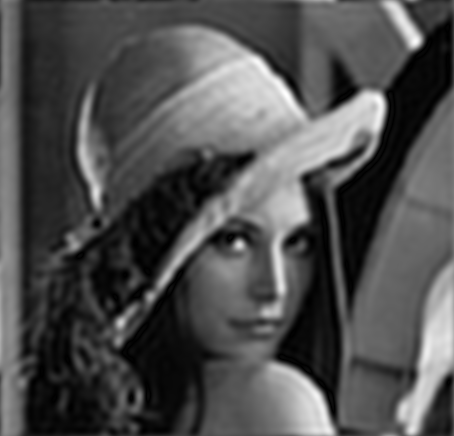
\includegraphics[width=55mm]{lena-deblurred-l010.png}};

\node at (-5.75,-11.0) {
\includegraphics[width=55mm]{lena-deblurred-l003.png}};
\node at ( 0   ,-11.0) {
\includegraphics[width=55mm]{lena-deblurred-l007.png}};
\node at ( 5.75,-11.0) {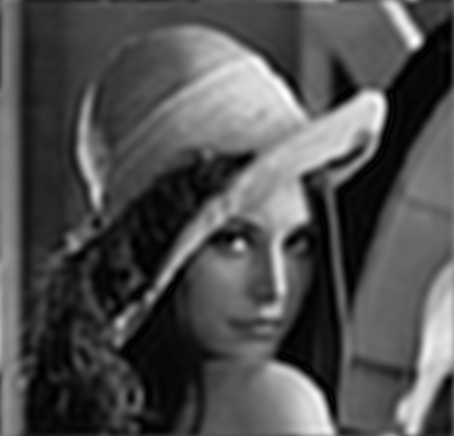
\includegraphics[width=55mm]{lena-deblurred-l011.png}};

\node at (-5.75,-16.5) {
\includegraphics[width=55mm]{lena-deblurred-l004.png}};
\node at ( 0   ,-16.5) {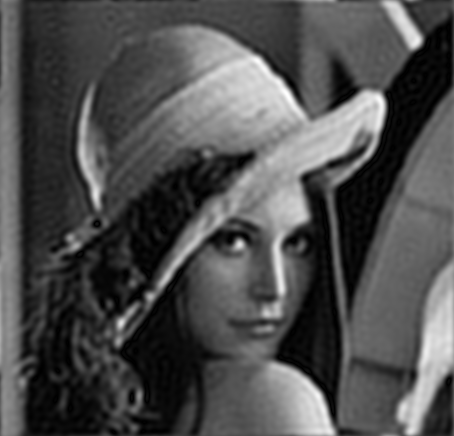
\includegraphics[width=55mm]{lena-deblurred-l008.png}};
\node at ( 5.75,-16.5) {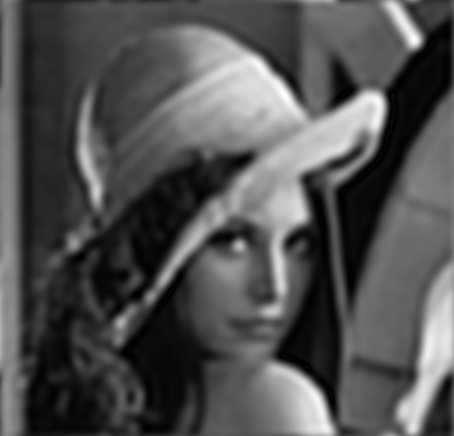
\includegraphics[width=55mm]{lena-deblurred-l012.png}};

\begin{scope}[xshift=-2.75cm,yshift=2.65cm]

\node[color=white] at (-5.75,0) [below right] {$K=0.01$};
\node[color=white] at (    0,0) [below right] {$K=0.16$};
\node[color=white] at ( 5.75,0) [below right] {$K=2.56$};

\node[color=white] at (-5.75,-5.5) [below right] {$K=0.02$};
\node[color=white] at ( 0   ,-5.5) [below right] {$K=0.32$};
\node[color=white] at ( 5.75,-5.5) [below right] {$K=5.12$};

\node[color=white] at (-5.75,-11.0) [below right] {$K=0.04$};
\node[color=white] at ( 0   ,-11.0) [below right] {$K=0.64$};
\node[color=white] at ( 5.75,-11.0) [below right] {$K=10.24$};

\node[color=white] at (-5.75,-16.5) [below right] {$K=0.08$};
\node[color=white] at ( 0   ,-16.5) [below right] {$K=1.28$};
\node[color=white] at ( 5.75,-16.5) [below right] {$K=20.48$};

\end{scope}


\end{tikzpicture}

\end{document}
